\chapter{Camera Calibration}
\label{ch:lesson27}

Chapter~\ref{ch:lesson26} introduced the camera intrinsics matrix $K$ to model a pinhole camera. The classic approach (\citelink{zhang2000}{Zhang, 2000}) to \textbf{camera calibration} recovers $K$ by showing the camera a known flat pattern (a checkerboard) from several different angles: extracting a homography (Chapter~\ref{ch:lesson24}) between the checkerboard plane and each image, then combining constraints from several such homographies to estimate $K$.

\section{What calibration recovers}

Camera calibration recovers two separate things:
\begin{enumerate}
  \item \textbf{Intrinsics} $K=\begin{bmatrix}f_x&s&c_x\\0&f_y&c_y\\0&0&1\end{bmatrix}$: focal lengths, principal point, and skew --- the ideal pinhole part of the camera model used throughout the next two chapters. Skew can safely be assumed zero for real cameras.
  \item \textbf{Distortion coefficients} $(k_1,k_2,p_1,p_2,k_3,\ldots)$: real lenses aren't perfect pinholes. Radial distortion ($k_1,k_2,k_3$) bows straight lines into curves (barrel or pincushion, depending on sign); tangential distortion ($p_1,p_2$) accounts for the lens not being perfectly parallel to the sensor.
\end{enumerate}
Every equation in the next two chapters secretly assumes a pinhole camera model --- i.e.\ that distortion has already been removed, which requires calibration.

\section{A synthetic calibration rig}

Create synthetic images of a camera viewing a checkerboard: define a ground-truth $K$ and distortion, define a flat checkerboard's 3D corner positions, and generate several ``photos'' of it from different poses by projecting the corners with \code{cv2.projectPoints} (which applies distortion exactly as a real lens would). This gives the same kind of input \code{cv2.calibrateCamera} expects from real detected checkerboard corners, while also providing ground truth to check against. Of 40 attempted random poses, $11$ land fully inside the frame and are usable.

\subsection*{Detecting the target}

A real calibration pipeline knows the checkerboard's own flat 2D layout, but not the board's pose in each shot, and not where its corners land in each photo --- so the first step is finding those 2D positions with \code{cv2.findChessboardCorners}, exactly as on a real photograph. Corners are detected in $8$ of the $11$ synthetic photos, with a mean per-view corner error of $1.83$ px (max $2.37$ px) against the ground truth --- realistic detector noise, not a bug. Figure~\ref{fig:l27-1} shows the target and one view's detections.

\begin{figure}[h]
\centering
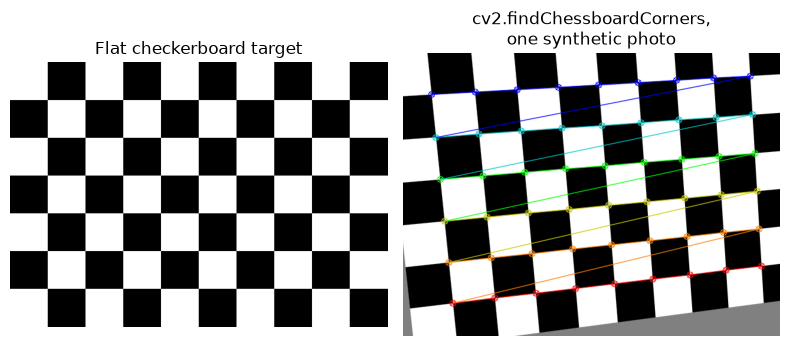
\includegraphics[width=0.75\textwidth]{figures/lesson27_fig01.png}
\caption{The flat checkerboard target, and \code{cv2.findChessboardCorners}' detections on one synthetic photo.}
\label{fig:l27-1}
\end{figure}

\section{Running calibration}

Zhang's calibration algorithm (\code{cv2.calibrateCamera}) takes the known corner positions on the checkerboard and their \emph{detected} 2D image positions across all views, and jointly solves for $K$, distortion, and each view's own pose. With only 8 noisy views: the RMS reprojection error comes to $0.264$ px, and $K$ is recovered reasonably close ($f_x=822.6$, $f_y=826.3$ vs.\ true $800, 800$) --- but the distortion coefficients drift much further from the true values ($k_1$ estimated at $0.0054$ vs.\ true $-0.3$). Using noisy corner detections, calibration does not recover the ground truth parameters exactly; this is why in practice you'd use as many views, from as wide a variety of angles, as practical --- more (and more diverse) constraints average out detector noise and better constrain the estimation, especially for distortion.

\section{Straight lines, bent by a lens}

Lens distortion causes straight lines to become curved. In normalized (pre-$K$) camera coordinates:
\begin{align}
x_d &= x(1+k_1r^2+k_2r^4+k_3r^6) + 2p_1xy + p_2(r^2+2x^2), \\
y_d &= y(1+k_1r^2+k_2r^4+k_3r^6) + p_1(r^2+2y^2) + 2p_2xy,
\end{align}
where $r^2=x^2+y^2$ --- exactly the model \code{cv2.projectPoints} applied internally above. Figure~\ref{fig:l27-2} shows the visible effect on a grid of straight lines.

\begin{figure}[h]
\centering
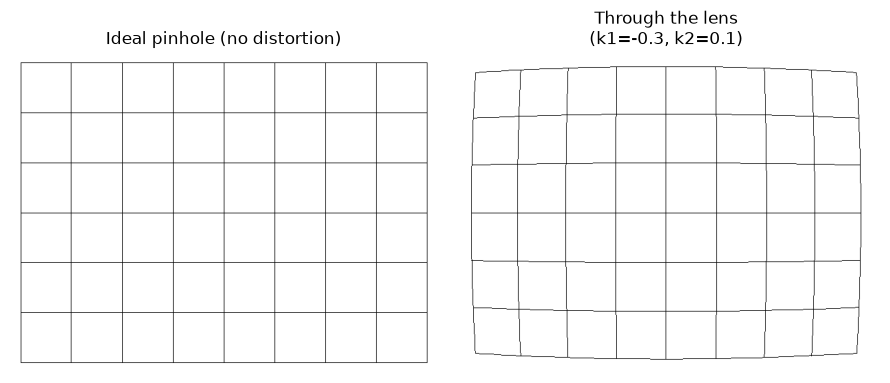
\includegraphics[width=0.9\textwidth]{figures/lesson27_fig02.png}
\caption{An ideal pinhole grid (straight lines) vs.\ the same grid through a lens with $k_1=-0.3$, $k_2=0.1$ --- visibly bowed.}
\label{fig:l27-2}
\end{figure}

\section{Undoing distortion with the estimated parameters}

\code{cv2.undistortPoints} inverts the distortion model, converting distorted pixel coordinates back to normalized undistorted coordinates. Applying it to the bent grid lines, using the \emph{estimated} (not the true) calibration, straightens them back out, with a max recovery error of $3.4\times10^{-2}$ in normalized coordinates (Figure~\ref{fig:l27-3}).

\begin{figure}[h]
\centering
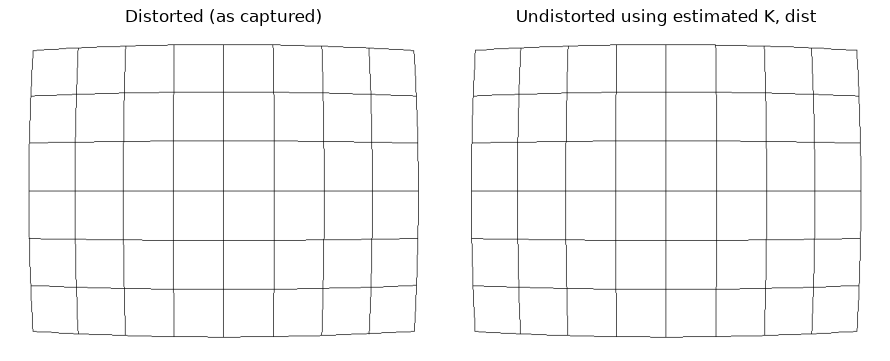
\includegraphics[width=0.9\textwidth]{figures/lesson27_fig03.png}
\caption{Distorted grid (as captured) vs.\ undistorted using the estimated $K$ and distortion --- the lines straighten out, though a faint bow remains, since the estimated parameters are themselves only approximately correct.}
\label{fig:l27-3}
\end{figure}

This process of calibrating a real camera should be performed, if possible, before handing real photos to any of the geometric machinery from the next two chapters, all of which implicitly assumes an ideal, distortion-free pinhole model. Keep in mind, however, that many modern pipelines perform auto-calibration without checkerboard images, using simplified camera models (typically just one focal length parameter --- ignoring aspect ratio, non-central principal point, and lens distortion).

\subsection*{Exercises}
\begin{enumerate}
  \item Add extra synthetic pixel noise (e.g.\ std $0.5$) on top of the real detector noise, to each view's detected corners before calibrating. How much does the RMS reprojection error grow, and how does the estimated $K$ drift further from the true one?
  \item This setup ends with only a handful of successfully-detected views. Try reducing that down to just 3 views before calibrating. Does the estimate noticeably degrade, especially for the distortion coefficients (which need corners spread widely across the frame, including near the edges, to be well constrained)?
  \item Set the true distortion to all zeros (a perfect pinhole) and rerun. Confirm the ``distorted'' and ``ideal'' grids become identical, and that calibration still recovers the true $K$ reasonably well even with zero distortion to estimate.
\end{enumerate}

\vfill
\fullcode{lesson27}{lesson27_camera_calibration}
